\documentclass[11pt,a4paper]{article}
\usepackage[T1]{fontenc}
\usepackage{lmodern,microtype}
\usepackage[margin=25mm]{geometry}
\usepackage{amsmath,amssymb,amsthm,mathtools}
\usepackage{booktabs,array,enumitem,xcolor,fancyhdr,needspace}
\usepackage{tikz,listings}
\usepackage[hypertexnames=false,colorlinks=true,linkcolor=blue!45!black,citecolor=blue!45!black,urlcolor=blue!45!black]{hyperref}
\setlength{\emergencystretch}{3em}
\setlength{\parskip}{0.25em}
\setlist{topsep=3pt,itemsep=3pt}
\pagestyle{fancy}\fancyhf{}
\fancyhead[L]{\small Robin eigenvalue nonconcavity on convex domains}
\fancyhead[R]{\small Research manuscript}
\fancyfoot[C]{\thepage}
\setlength{\headheight}{14pt}
\newtheorem{theorem}{Theorem}[section]
\newtheorem{lemma}[theorem]{Lemma}
\newtheorem{proposition}[theorem]{Proposition}
\newtheorem{corollary}[theorem]{Corollary}
\theoremstyle{definition}\newtheorem{definition}[theorem]{Definition}
\theoremstyle{remark}\newtheorem{remark}[theorem]{Remark}
\newcommand{\R}{\mathbb R}
\newcommand{\N}{\mathbb N}
\newcommand{\dd}{\,\mathrm d}
\newcommand{\norm}[1]{\left\lVert#1\right\rVert}
\DeclareMathOperator{\spanop}{span}
\DeclareMathOperator{\spec}{spec}
\lstset{basicstyle=\ttfamily\scriptsize,breaklines=true,columns=fullflexible,
 keepspaces=true,showstringspaces=false,frame=single,
 rulecolor=\color{black!25},xleftmargin=3pt,xrightmargin=3pt,
 aboveskip=8pt,belowskip=8pt}
\title{Nonconcavity of Robin Eigenvalues\\on Convex Trapezoids\\[5pt]
\large An affine-width counterexample to Laugesen's Conjecture C}
\author{Keio Research Notes}
\date{31 October 2026}
\hypersetup{pdftitle={Nonconcavity of Robin Eigenvalues on Convex Trapezoids},pdfauthor={Keio Research Notes},pdfsubject={An unconditional counterexample to Laugesen's positive-parameter second Robin eigenvalue concavity conjecture}}
\begin{document}
\maketitle
\begin{abstract}
We construct bounded convex planar domains for which the second
Robin eigenvalue is not concave in the positive boundary parameter,
giving a negative answer to Conjecture C of Laugesen (2019).
The domains are thin trapezoids of width $2\varepsilon(1+\delta x)$.
With Robin parameter $\alpha=\varepsilon t$, their low eigenvalues
converge to a weighted Neumann problem on the unit interval.
For its $(n+1)$st eigenvalue, $n\geq1$, we prove the exact response
\[
 \partial_t^2\Lambda_{n+1}(\delta,t)
 =\frac{n^2\pi^2+21}{24n^4\pi^4}\,\delta^2+O(\delta^3),
\]
uniformly on each fixed compact $t$-interval. The coefficient is
positive. A strict midpoint defect at $t=1,2,3$ therefore transfers
to the original Robin problem at $\alpha=\varepsilon,2\varepsilon,
3\varepsilon$ on one fixed convex domain. For every prescribed
finite $M$, the same domain and parameters work simultaneously for
the eigenvalues $\lambda_2,\ldots,\lambda_M$. We also establish a
general width-profile response formula, stability under nearby
concave profiles, and extensions to real-analytic strictly convex domains in every
dimension at least two. The proofs are
analytic and use neither an unproved conjecture nor a numerical
sign certificate. Variational convergence and eigenvalue
perturbation are established tools; the contribution is their
explicit affine-width application to the stated concavity problem.
\end{abstract}

\section{The original problem and the main result}
\label{sec:introduction}

For a bounded Lipschitz domain $\Omega\subset\R^d$, let
$\lambda_j(\Omega;\alpha)$ be the Robin eigenvalues, counted with
multiplicity and starting at $j=1$, with outward-normal convention
\begin{equation}\label{eq:robin-problem}
 -\Delta u=\lambda u\quad\text{in }\Omega,
 \qquad \partial_\nu u+\alpha u=0\quad\text{on }\partial\Omega.
\end{equation}
The scalar parameter $\alpha$ is constant on the entire boundary.
Equivalently these are the eigenvalues of the closed quadratic form
\begin{equation}\label{eq:robin-form}
 q_{\Omega,\alpha}[u]
 =\int_\Omega|\nabla u|^2\,dx
       +\alpha\int_{\partial\Omega}|u|^2\,dS,
 \qquad u\in H^1(\Omega),
\end{equation}
in $L^2(\Omega)$. The first eigenvalue is concave in $\alpha$ by
the Rayleigh principle. The question for the second eigenvalue is
different because its variational characterization is a min--max.

Laugesen's Conjecture C \cite[Section~2, p.~7]{Laugesen2019}
asserts that every bounded convex $\Omega$ has
\begin{equation}\label{eq:original-conjecture}
 \alpha\longmapsto\lambda_2(\Omega;\alpha)
 \quad\text{concave on }(0,\infty).
\end{equation}
It is also listed in the 2020 eigenvalue miniconference
\cite[Open Problem~7]{Eigenvalues2020} and in the 2023 Oberwolfach
report \cite[p.~2099]{OWR2023}. The result below concerns this
original positive-parameter, convex-domain statement.

For $\varepsilon,\delta>0$, set
\begin{equation}\label{eq:trapezoid}
 \Omega_{\varepsilon,\delta}
 =\{(x,y)\in\R^2:0<x<1,\ |y|<\varepsilon(1+\delta x)\}.
\end{equation}
This is the intersection of four open half-planes, hence is a
bounded open convex trapezoid with Lipschitz boundary. Define its
midpoint defect by
\begin{equation}\label{eq:physical-defect}
 D_j(\varepsilon,\delta)
 =\lambda_j(\Omega_{\varepsilon,\delta};\varepsilon)
  +\lambda_j(\Omega_{\varepsilon,\delta};3\varepsilon)
  -2\lambda_j(\Omega_{\varepsilon,\delta};2\varepsilon).
\end{equation}
A concave eigenvalue curve would require $D_j\leq0$.

\begin{theorem}[Convex-domain nonconcavity]\label{thm:main}
For every integer $M\geq2$ there is a number $\delta_M>0$ such
that for every $\delta\in(0,\delta_M)$ there exists
$\varepsilon_0(\delta,M)>0$ for which
\begin{equation}\label{eq:main-defect}
 D_j(\varepsilon,\delta)>0
 \qquad(0<\varepsilon<\varepsilon_0(\delta,M),\ 2\leq j\leq M).
\end{equation}
In particular, Conjecture~\eqref{eq:original-conjecture} is false.
For each fixed $j\geq2$, the precise iterated limit is
\begin{equation}\label{eq:main-iterated-limit}
 \lim_{\delta\downarrow0}\frac1{\delta^2}
       \lim_{\varepsilon\downarrow0}D_j(\varepsilon,\delta)
 =\frac{(j-1)^2\pi^2+21}{24(j-1)^4\pi^4}>0.
\end{equation}
\end{theorem}

All parameters are positive. After selecting $\delta$ and
$\varepsilon$, the three eigenvalues in
\eqref{eq:physical-defect} are evaluated on the same domain.
The two limits in \eqref{eq:main-iterated-limit} are taken in the
displayed order; no estimate uniform in all $j$ is asserted.
The proof establishes an open range of sufficiently small positive
parameters, rather than an unverified decimal example.

\begin{figure}[ht]
\centering
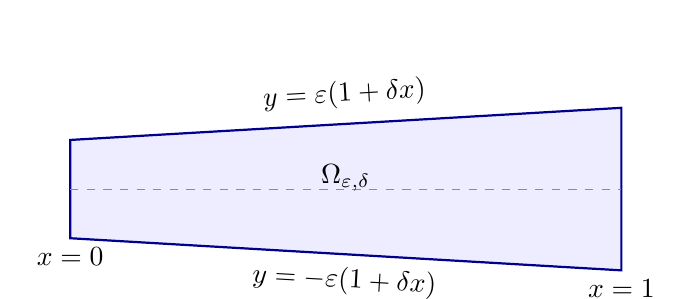
\begin{tikzpicture}[x=7.0cm,y=1.2cm,>=stealth]
 \fill[blue!7] (0,-0.52)--(1,-0.86)--(1,0.86)--(0,0.52)--cycle;
 \draw[thick,blue!55!black] (0,-0.52)--(1,-0.86)--(1,0.86)--(0,0.52)--cycle;
 \draw[dashed,black!45] (0,0)--(1,0);
 \node[below] at (0,-0.52) {$x=0$};
 \node[below] at (1,-0.86) {$x=1$};
 \node[above,rotate=3.3] at (0.5,0.75) {$y=\varepsilon(1+\delta x)$};
 \node[below,rotate=-3.3] at (0.50,-0.72) {$y=-\varepsilon(1+\delta x)$};
 \node at (0.50,0.12) {$\Omega_{\varepsilon,\delta}$};
\end{tikzpicture}
\caption{The convex trapezoid. Vertical scale is exaggerated.
The same Robin parameter is imposed on all four sides.}
\label{fig:trapezoid}
\end{figure}

\subsection{How the proof is organized}
The argument has three ingredients. First, the scaling
$\alpha=\varepsilon t$ converts the boundary term of a thin domain
into an effective multiplication operator on an interval.
Second, a reduced-resolvent identity isolates the exact quadratic
effect of changing the width. Third, a finite midpoint inequality
passes through eigenvalue convergence. This last step avoids
differentiating a thin-domain limit.

The main construction uses only the affine profile $x\mapsto x$.
We first prove a response formula for general Lipschitz profiles
to identify which part of the calculation controls the sign.
The full proofs include the change in the weighted Hilbert space,
all boundary faces, and the ordering of eigenvalues.

\subsection{Provenance and scope}
The source problem is independent of the supplied
Verifiable Mathematical Reasoning Corpus \cite{VMRC}. We checked
the 95 TeX manuscripts in its 29 October 2026 snapshot and found no
instance of the present positive-parameter concavity counterexample.
The corpus and earlier research notes motivated the search for
exact finite certificates and for transfers that preserve the
original quantifiers. The present proof does not assume any
unverified corpus theorem or any arithmetic statement about
Euler's constant.

The mathematical theorem and a claim of historical priority are
separate matters. Section~\ref{sec:status} records the primary
sources examined and the limits of the novelty audit. This is a
research manuscript prepared with AI assistance, not a report of
external peer review.

\section{Thin convex domains and an effective boundary potential}

For a positive Lipschitz function $h:[0,1]\to(0,\infty)$ and
$\varepsilon>0$, put
\[
 \Omega_{\varepsilon,h}
 =\{(x,y):0<x<1,\ -\varepsilon h(x)<y<\varepsilon h(x)\}.
\]
If $h$ is concave, $\Omega_{\varepsilon,h}$ is convex. Its Robin
eigenvalues $\lambda_j(\Omega_{\varepsilon,h};\alpha)$ correspond to
$\partial_\nu u+\alpha u=0$ on the whole boundary and are numbered
starting at $j=1$. Define $\Lambda_j(h,t)$ by the regular weighted
Sturm--Liouville form
\begin{equation}\label{eq:effective-form}
 a_{h,t}[u]=\int_0^1h(x)|u'(x)|^2\,dx
              +t\int_0^1|u(x)|^2\,dx,
 \qquad u\in H^1(0,1),
\end{equation}
in $L^2((0,1),h\,dx)$. Thus the endpoint conditions are Neumann and
the equation is
\[
 -(hu')'+tu=\Lambda hu,\qquad u'(0)=u'(1)=0.
\]

\begin{lemma}[Thin-domain convergence]\label{lem:thin-convergence}
For every positive Lipschitz $h$, every $t\geq0$, and every fixed
$j\geq1$,
\begin{equation}\label{eq:thin-limit}
 \lim_{\varepsilon\downarrow0}
 \lambda_j(\Omega_{\varepsilon,h};\varepsilon t)
 =\Lambda_j(h,t).
\end{equation}
\end{lemma}

\begin{proof}
On $D=(0,1)\times(-1,1)$ make the change of variables
$F_\varepsilon(x,s)=(x,\varepsilon h(x)s)$ and write
$v=u\circ F_\varepsilon$. After division of the numerator and
denominator of the Rayleigh quotient by $\varepsilon$, the squared
norm becomes
\[
 m[v]=\int_D h(x)|v(x,s)|^2\,dx\,ds,
\]
and its numerator is exactly
\begin{align}
 q_{\varepsilon,t}[v]
 &=\int_D h\left|v_x-\frac{h'}h s v_s\right|^2\,dx\,ds
  +\varepsilon^{-2}\int_Dh^{-1}|v_s|^2\,dx\,ds\notag\\
 &\quad+t\int_0^1\sqrt{1+\varepsilon^2h'(x)^2}
       \bigl(|v(x,1)|^2+|v(x,-1)|^2\bigr)\,dx\notag\\
 &\quad+\varepsilon t\sum_{r\in\{0,1\}}h(r)
                   \int_{-1}^1|v(r,s)|^2\,ds.
 \label{eq:exact-pullback}
\end{align}
Every term is nonnegative. For functions independent of $s$,
$m[v]=2\int h|u|^2$ and $q_{\varepsilon,t}[v]\to2a_{h,t}[u]$.
The convergence is uniform on each fixed finite-dimensional subspace
of $H^1(0,1)$. Applying the minimax principle to the span of the
first $j$ effective eigenfunctions proves the upper bound in
\eqref{eq:thin-limit}.

For the lower bound, take a sequence along which the lower limit
of the $j$th eigenvalue is attained, and choose $m$-orthonormal
eigenfunctions $v_{\varepsilon,1},\ldots,v_{\varepsilon,j}$ for the
first $j$ eigenvalues. The upper bound controls their forms. The
second term in \eqref{eq:exact-pullback} gives
$\|\partial_sv_{\varepsilon,k}\|_{L^2(D)}=O(\varepsilon)$.
Since $h$ is bounded above and below and $h'$ is bounded, the first
term then bounds $\partial_xv_{\varepsilon,k}$ in $L^2(D)$.
Consequently these functions are bounded in $H^1(D)$. After a
subsequence they converge weakly in $H^1(D)$, strongly in $L^2(D)$,
and their limits are independent of $s$ and remain
$m$-orthonormal. To justify the boundary terms directly, put
$\bar v(x)=\tfrac12\int_{-1}^1v(x,s)\,ds$. For almost every $x$,
\[
 |v(x,\pm1)-\bar v(x)|^2
 \leq2\int_{-1}^1|v_s(x,s)|^2\,ds.
\]
Thus the two sloping-side traces converge strongly in $L^2(0,1)$
to the same limiting longitudinal function. The endpoint
boundary terms need no convergence assertion for the lower bound.

For every fixed linear combination of these $j$ functions, weak
lower semicontinuity applies to the longitudinal term; the
top and bottom traces converge strongly; and the transverse and
endpoint terms may be discarded. The corresponding effective
Rayleigh quotient is therefore at most the lower limit of the
$j$th eigenvalue. The limit functions span a $j$-dimensional space,
so a second application of minimax proves the reverse bound.
\end{proof}

\section{A curvature response for width profiles}

Let $f\in W^{1,\infty}(0,1)$ be real, set $h_\delta=1+\delta f$,
and restrict $\delta$ to a neighborhood of zero where $h_\delta>0$.
Write $\Lambda_j(\delta,t)=\Lambda_j(h_\delta,t)$. On unweighted
$L^2(0,1)$, let
\[
 E_n=n^2\pi^2,\qquad \phi_0=1,\qquad
 \phi_n(x)=\sqrt2\cos(n\pi x)\quad(n\geq1).
\]
These are the eigenpairs of the Neumann Laplacian $A_0$. Let
$P_n$ be the orthogonal projection onto $\phi_n$ and define the
bounded reduced resolvent
\[
 R_n=(1-P_n)(E_n-A_0)^{-1}(1-P_n),
\]
where the inverse is taken only on the orthogonal complement.
For a real bounded function $f$, define
\begin{equation}\label{eq:profile-response}
 \mathcal Q_n(f)=2\langle f\phi_n,R_n f\phi_n\rangle
 =2\sum_{m\ne n}
  \frac{|\langle f\phi_n,\phi_m\rangle|^2}{E_n-E_m}.
\end{equation}
The series is absolutely convergent: the reduced resolvent is
bounded and the squared Fourier coefficients are summable.


\paragraph{An auxiliary design question.}
Can one choose a single nonconstant concave profile $f$ such that
$\mathcal Q_n(f)>0$ for every $n\geq1$, while
$\mathcal Q_0(f)<0$? This is a design problem for the limiting
response, introduced here to find counterexamples to the original
Robin conjecture. Lemma~\ref{lem:linear-response} answers it with
the affine profile $f(x)=x$. The all-index assertion concerns
the response coefficients; transfer to one physical domain below
is asserted only for a prescribed finite set of eigenvalues.
\begin{lemma}[Simple-eigenvalue curvature]\label{lem:curvature-identity}
Let $H(s)=H_*+sC$ be a self-adjoint family with compact resolvent,
where $C$ is bounded and self-adjoint. Suppose $e(s)$ is a simple
eigenvalue with normalized real eigenvector $\psi(s)$. Write $P$
for its eigenprojection and
\[
 R=(1-P)(e(s)-H(s))^{-1}(1-P)
\]
for the inverse on the orthogonal complement. Then
\begin{equation}\label{eq:curvature-identity}
 e''(s)=2\langle C\psi(s),R C\psi(s)\rangle.
\end{equation}
Replacing $C$ by $C-cI$ on the right does not change the result.
\end{lemma}
\begin{proof}
Choose the real normalization with
$\langle\psi,\psi'\rangle=0$. Differentiating the eigenvalue
equation gives
\[
 e'=\langle C\psi,\psi\rangle,\qquad
 (e-H)\psi'=(C-e')\psi.
\]
The latter identity on the orthogonal complement yields
$\psi'=RC\psi$. Differentiating the first identity proves
\eqref{eq:curvature-identity}. Since $R\psi=0$ and $R$ is
self-adjoint, scalar multiples of the identity disappear.
Existence of the derivatives follows from the isolated simple
eigenvalue and the resolvent Neumann series; this is the standard
simple-eigenvalue perturbation argument \cite[Chapter~VII]{Kato}.
\end{proof}
\begin{lemma}[Uniform width-profile curvature]
\label{lem:profile-curvature-uniform}
Let $f\in W^{1,\infty}(0,1)$ be real, let $h_\delta=1+\delta f$,
and let $\Lambda_j(\delta,t)$ be the eigenvalues of
\eqref{eq:effective-form} with this weight. For every $T>0$ and
integer $N\geq0$,
\begin{equation}\label{eq:uniform-curvature}
 \lim_{\delta\to0}\max_{0\leq n\leq N}\ 
 \sup_{0\leq t\leq T}
 \left|\delta^{-2}\partial_t^2\Lambda_{n+1}(\delta,t)
                      -\mathcal Q_n(f)\right|=0,
\end{equation}
where $\mathcal Q_n$ is defined by \eqref{eq:profile-response}.
More precisely, for these fixed $T,N,f$, the supremum in
\eqref{eq:uniform-curvature} is $O(|\delta|)$; hence
\begin{equation}\label{eq:uniform-expansion}
 \partial_t^2\Lambda_{n+1}(\delta,t)
 =\delta^2\mathcal Q_n(f)+O(\delta^3)
 \quad(0\leq t\leq T,\ 0\leq n\leq N).
\end{equation}
The derivatives in this statement exist for every sufficiently
small $|\delta|$, uniformly on the indicated compact interval.
\end{lemma}

\begin{proof}
Under the unitary map $u\mapsto\sqrt{h_\delta}\,u$, the effective
operator is $A_\delta+tV_\delta$, where $A_\delta$ is associated
with the common-domain form
\[
 b_\delta[g]=\int_0^1\left|g'
       -\frac{\delta f'}{2(1+\delta f)}g\right|^2\,dx,
       \qquad g\in H^1(0,1),
\]
and $V_\delta$ is multiplication by $(1+\delta f)^{-1}$. Define
\[
 W_\delta=\frac{V_\delta-I}{\delta}
             =-\frac{f}{1+\delta f},\qquad
 B_{\delta,t}=A_\delta+t(V_\delta-I).
\]
The eigenvalues of $B_{\delta,t}$ are
$\Lambda_j(\delta,t)-t$. This subtraction leaves all spectral
gaps and all second derivatives in $t$ unchanged.

The forms of $B_{\delta,t}$ converge to the Neumann form
$b_0[g]=\int|g'|^2$ in form norm, uniformly for $0\leq t\leq T$.
Indeed, their difference is bounded in absolute value by
$C_T|\delta|\|g\|_{H^1}^2$. After adding a fixed sufficiently
large positive multiple of $\|g\|_{L^2}^2$, these forms are
uniformly coercive. The variational resolvent identity then gives
norm-resolvent convergence uniform in $t$, with error $O(|\delta|)$.
Explicitly, regard the shifted forms as bounded invertible maps
$H^1\to(H^1)^*$ and apply
$L_\delta^{-1}-L_0^{-1}
=L_\delta^{-1}(L_0-L_\delta)L_0^{-1}$.
The continuous embeddings from $L^2$ to $(H^1)^*$ and from
$H^1$ to $L^2$ give the claimed operator-norm estimate.
The resolvent identity propagates it to any fixed compact contour
in the resolvent set of $A_0$. Since the finitely
many Neumann eigenvalues $E_0,\ldots,E_N$ are isolated and simple,
fixed disjoint small circles around them give spectral
projections converging in norm, uniformly in $t$. In particular,
the corresponding normalized real eigenfunctions
$\psi_{n,\delta,t}$ may be chosen with
\[
 \sup_{0\leq t\leq T}\|\psi_{n,\delta,t}-\phi_n\|_{L^2}\to0.
\]
Their reduced resolvents $R_{n,\delta,t}$ converge in operator
norm to $R_n$, also uniformly in $t$. All of these convergences have error $O(|\delta|)$.
For the reduced resolvent this follows, for example, from
\[
 R_{n,\delta,t}=\frac{1}{2\pi i}
 \int_{\Gamma_n}\frac{(z-B_{\delta,t})^{-1}}
                        {z-e_{n,\delta,t}}\,dz,
 \qquad e_{n,\delta,t}=\Lambda_{n+1}(\delta,t)-t,
\]
where $\Gamma_n$ is a fixed small positively oriented circle
enclosing only this eigenvalue. The eigenprojection contribution
has a double pole of zero contour integral; every other spectral
component has residue $(e_{n,\delta,t}-e_m)^{-1}$. Simplicity on a neighborhood of the compact
parameter interval and the common analytic form domain justify
ordinary simple-eigenvalue differentiation.

Because $\partial_tB_{\delta,t}=V_\delta-I=\delta W_\delta$,
Lemma~\ref{lem:curvature-identity} gives the exact
identity
\[
 \delta^{-2}\partial_t^2\Lambda_{n+1}(\delta,t)
 =2\langle W_\delta\psi_{n,\delta,t},
          R_{n,\delta,t}W_\delta\psi_{n,\delta,t}\rangle.
\]
Finally $W_\delta\to-f$ in multiplication-operator norm. The
uniform convergence, with error $O(|\delta|)$, of all three
factors on the right proves
\eqref{eq:uniform-curvature}. Taking a maximum over finitely
many $n$ does not affect convergence.
\end{proof}

\section{An exact calculation for affine width}

\begin{lemma}[Linear-profile response]\label{lem:linear-response}
For $f(x)=x$,
\begin{equation}\label{eq:linear-curvature}
 \mathcal Q_0(x)=-\frac1{60},\qquad
 \mathcal Q_n(x)=\frac{n^2\pi^2+21}{24n^4\pi^4}>0
       \quad(n\geq1).
\end{equation}
\end{lemma}

\begin{proof}
Fix $n\geq1$, put $k=n\pi$, and define
\[
 y_n(x)=\sqrt2\left[
 \left(\frac{x^2-x}{4k}-\frac1{4k^3}\right)\sin(kx)
       +\frac{x-1/2}{4k^2}\cos(kx)\right].
\]
Direct differentiation gives
\[
 y_n''+k^2y_n=(x-1/2)\phi_n,\quad
 y_n'(0)=y_n'(1)=0,\quad
 \int_0^1y_n\phi_n\,dx=0.
\]
Since $\int_0^1x\phi_n^2\,dx=1/2$, these identities characterize
$y_n=R_nx\phi_n$. Integration by parts gives
\begin{align*}
 \int_0^1x(x^2-x)\cos(kx)\sin(kx)\,dx&=\frac3{8k^3},\\
 \int_0^1x(x-1/2)\cos^2(kx)\,dx&=\frac1{24}+\frac1{4k^2},\\
 \int_0^1x\cos(kx)\sin(kx)\,dx&=-\frac1{4k}.
\end{align*}
It follows that
\[
 \langle x\phi_n,y_n\rangle
 =\frac1{48k^2}+\frac7{16k^4},
\]
which proves the second formula in \eqref{eq:linear-curvature}.
For $n=0$, the corresponding correction is
$y_0(x)=x^3/6-x^2/4+1/24$; it has mean zero and satisfies
$y_0''=x-1/2$ and the Neumann endpoint conditions. Hence
$\mathcal Q_0(x)=2\int_0^1xy_0\,dx=-1/60$.
\end{proof}


\section{A fixed finite defect and the original conjecture}
\begin{lemma}[A fixed three-point defect]\label{lem:fixed-defect}
For every fixed $n\geq0$ and real $f\in W^{1,\infty}(0,1)$,
\begin{equation}\label{eq:fixed-defect-limit}
 \lim_{\delta\to0}\frac{
 \Lambda_{n+1}(\delta,1)+\Lambda_{n+1}(\delta,3)
                      -2\Lambda_{n+1}(\delta,2)}{\delta^2}
 =\mathcal Q_n(f).
\end{equation}
\end{lemma}

\begin{proof}
For every twice continuously differentiable $F$ on $[1,3]$,
\[
 F(1)+F(3)-2F(2)
  =\int_1^2(t-1)F''(t)\,dt
     +\int_2^3(3-t)F''(t)\,dt.
\]
The two nonnegative weights have total integral one. Apply
Lemma~\ref{lem:profile-curvature-uniform} with $T=3$.
\end{proof}

\begin{theorem}[Convex trapezoids with fixed parameter ratios]
\label{thm:fixed-ratio-trapezoids}
For every integer $M\geq2$, put
\[
 c_M=\frac{(M-1)^2\pi^2+21}{24(M-1)^4\pi^4}>0.
\]
There is $\delta_M\in(0,1)$ such that, for every
$\delta\in(0,\delta_M)$, there is
$\varepsilon_M(\delta)>0$ for which every
$0<\varepsilon<\varepsilon_M(\delta)$ satisfies
\begin{align}
 &\lambda_j(\Omega_{\varepsilon,\delta};\varepsilon)
 +\lambda_j(\Omega_{\varepsilon,\delta};3\varepsilon)
 -2\lambda_j(\Omega_{\varepsilon,\delta};2\varepsilon)
 >\frac14c_M\delta^2,
 \quad 2\leq j\leq M,\label{eq:quantitative-midpoint}\\[-2mm]
 &\Omega_{\varepsilon,\delta}
 =\{(x,y):0<x<1,\ |y|<\varepsilon(1+\delta x)\}.
 \notag
\end{align}
Consequently one fixed convex planar domain simultaneously
violates concavity of the first $M-1$ excited Robin eigenvalues,
at the same three positive parameters $\varepsilon,2\varepsilon,
3\varepsilon$.
\end{theorem}

\begin{proof}
Take $f(x)=x$. The exact formula
\eqref{eq:linear-curvature} decreases with $n\geq1$, so
$c_M=\min_{1\leq n<M}\mathcal Q_n(x)$. By
Lemma~\ref{lem:fixed-defect}, a common $\delta_M>0$ can be chosen
so that every effective defect for $j=2,\ldots,M$ is greater than
$c_M\delta^2/2$, whenever $0<\delta<\delta_M$. Fix such a
$\delta$. Lemma~\ref{lem:thin-convergence} applies at the finitely
many pairs $(j,t)$ with $2\leq j\leq M$ and $t\in\{1,2,3\}$.
For sufficiently small $\varepsilon$, every eigenvalue error
there is less than $c_M\delta^2/16$. The error of a three-point
defect is then less than $c_M\delta^2/4$, proving
\eqref{eq:quantitative-midpoint}.
\end{proof}


\begin{proof}[Completion of the proof of Theorem~\ref{thm:main}]
The strict inequality \eqref{eq:main-defect} follows from
Theorem~\ref{thm:fixed-ratio-trapezoids}. For each fixed $\delta$,
Lemma~\ref{lem:thin-convergence} identifies the inner limit in
\eqref{eq:main-iterated-limit} with the effective three-point
defect. Lemma~\ref{lem:fixed-defect} and
Lemma~\ref{lem:linear-response} then give the stated outer limit.
For $j=2$, the resulting strict defect contradicts the midpoint
inequality required by \eqref{eq:original-conjecture}.
\end{proof}

\begin{remark}[Why the limit order is sufficient]
Let $\Delta_j(\delta)$ denote the effective defect. For a chosen
$\delta$ the proof establishes $\Delta_j(\delta)>0$. Choose
$\varepsilon$ only after this step, so that each of the three
eigenvalue errors is less than $\Delta_j(\delta)/8$.
The error of the defect is then less than $\Delta_j(\delta)/2$.
This is a finite convergence argument, not an exchange of
derivatives or limits. The explicit positive lower bound
\eqref{eq:quantitative-midpoint} uses a common version of the
same estimate for finitely many indices.
\end{remark}
\section{Which width changes produce the positive sign?}
\label{sec:profiles}

The response formula separates the width calculation from the
thin-domain limit. Its sign is an indefinite spectral quadratic
form, rather than an automatic consequence of positivity of the
boundary form.

\begin{proposition}[Affine profiles and reflection-symmetric profiles]
\label{prop:profile-signs}
For every $n\geq0$ and real constants $a,b$,
\[
 \mathcal Q_n(a+bx)=b^2\mathcal Q_n(x).
\]
If $f\in L^\infty(0,1)$ is real, not almost everywhere constant,
and $f(1-x)=f(x)$ almost everywhere, then
\[
 \mathcal Q_1(f)<0.
\]
For every nonconstant real bounded profile,
$\mathcal Q_0(f)<0$.
\end{proposition}
\begin{proof}
Since $R_n\phi_n=0$, addition of a constant to $f$ does not
change $\mathcal Q_n$, and homogeneity gives the affine identity.
For $n=0$ every nonzero summand has a negative denominator.
Equality would force $f\phi_0$ to lie in the span of $\phi_0$,
which means that $f$ is constant.

For the second assertion, $\phi_1$ is odd under $x\mapsto1-x$.
Thus $f\phi_1$ is odd and is orthogonal to $\phi_0$, as well as
to all even-index cosine modes. The only positive-denominator
term in $\mathcal Q_1$ is the $\phi_0$ term, which vanishes.
All remaining terms, other than the omitted $\phi_1$ term, have
negative denominators. If they all vanished, completeness of the
cosine basis would give $f\phi_1=c\phi_1$ almost everywhere.
Since $\phi_1$ is nonzero except at one point, this again forces
$f$ to be constant.
\end{proof}

The affine width breaks reflection symmetry in the longitudinal
coordinate. The trapezoid still has a transverse reflection
symmetry, but its low excited modes are longitudinal; that
symmetry does not remove their coupling to the ground mode.
This is consistent with the symmetry mechanism discussed in
\cite{Laugesen2019}.

\begin{proposition}[An explicit neighborhood of useful profiles]
\label{prop:profile-neighborhood}
For $M\geq2$, put
\[
 q_n=\frac{n^2\pi^2+21}{24n^4\pi^4},\qquad
 g_n=(2n-1)\pi^2\quad(n\geq1),\qquad
 \eta_M=\min\left\{1,\min_{1\leq n<M}\frac{g_nq_n}{12}\right\}.
\]
If $f$ is real and $\|f-x\|_\infty<\eta_M$, then
$\mathcal Q_n(f)>q_n/2$ for $1\leq n<M$.
Consequently every concave $f\in W^{1,\infty}(0,1)$ in this
neighborhood produces the simultaneous concavity violations of
Theorem~\ref{thm:main}, on the convex domains
$\Omega_{\varepsilon,1+\delta f}$, for sufficiently small
$\delta>0$ and then sufficiently small $\varepsilon>0$.
\end{proposition}
\begin{proof}
The spectral distance of $E_n$ from the other Neumann eigenvalues
is $g_n$, so $\|R_n\|=1/g_n$. Expanding the difference of the two
quadratic forms gives
\[
 |\mathcal Q_n(f)-\mathcal Q_n(x)|
 \leq\frac{2}{g_n}\|f-x\|_\infty(\|f\|_\infty+\|x\|_\infty)
 \leq\frac{6}{g_n}\|f-x\|_\infty.
\]
The chosen neighborhood makes the last quantity less than $q_n/2$.
Use Lemma~\ref{lem:fixed-defect} for these finitely many positive
responses and then Lemma~\ref{lem:thin-convergence}. Concavity of
$f$ and positivity of $1+\delta f$ give convexity of the domain.
The threshold for $\delta$ may depend on $f$, including its
Lipschitz constant.
\end{proof}

\section{Higher-dimensional convex polytopes}
\begin{corollary}[Every ambient dimension]
\label{cor:all-dimensions}
For every $d\geq2$ and $M\geq2$, there are bounded convex
polytopes in $\mathbb R^d$ and positive parameters
$\alpha,2\alpha,3\alpha$ for which
\[
 \lambda_j(\Omega;\alpha)+\lambda_j(\Omega;3\alpha)
      >2\lambda_j(\Omega;2\alpha),\qquad 2\leq j\leq M.
\]
One may use the explicit family
\begin{equation}\label{eq:product-polytopes}
 \Omega_{\varepsilon,\delta}^{(d,M)}
 =\Omega_{\varepsilon,\delta}\times(0,1/(2M))^{d-2},
 \qquad \alpha=\varepsilon,
\end{equation}
with $\delta>0$ sufficiently small and then $\varepsilon>0$
sufficiently small. The empty Cartesian factor for $d=2$ is
understood.
\end{corollary}

\begin{proof}
The planar assertion has already been proved. Fix $d\geq3$ and
write $\ell=1/(2M)$. Let $\eta_k(\alpha)$ denote the Robin
eigenvalues of $(0,\ell)$, starting with $k=1$. The Robin form
on a Cartesian product separates, so its complete spectrum is
formed by sums of the spectra of the factors. Since
\[
 \eta_1(\varepsilon t)\to0,\qquad
 \eta_2(\varepsilon t)-\eta_1(\varepsilon t)
                  \to\pi^2/\ell^2=4M^2\pi^2
\]
for each fixed $t\geq0$, excitation of an extra interval factor
has a uniformly large limiting cost at $t\in\{1,2,3\}$.

To check that the first $M$ eigenvalues arise from planar
excitations, take $0<\delta<1$. Directly from the effective
Rayleigh quotient and $1\leq h_\delta\leq1+\delta$,
\[
 \frac{(j-1)^2\pi^2+t}{1+\delta}
 \leq\Lambda_j(\delta,t)
 \leq(1+\delta)(j-1)^2\pi^2+t.
\]
Hence for $1\leq t\leq3$,
\[
 \Lambda_M(\delta,t)-\Lambda_1(\delta,t)
 \leq2(M-1)^2\pi^2+\frac32
 <4M^2\pi^2.
\]
The planar thin-domain limit preserves this strict separation
for all sufficiently small $\varepsilon$, simultaneously at
$t=1,2,3$. Thus for $1\leq j\leq M$ at these parameters,
\[
 \lambda_j(\Omega_{\varepsilon,\delta}^{(d,M)};
                    \varepsilon t)
 =\lambda_j(\Omega_{\varepsilon,\delta};\varepsilon t)
                  +(d-2)\eta_1(\varepsilon t).
\]
For fixed $d$, the extra term tends to zero. Consequently each
product-domain midpoint defect has exactly the same positive
limit as its planar effective defect. Choose $\delta$ as in
Theorem~\ref{thm:fixed-ratio-trapezoids}, and then take
$\varepsilon$ sufficiently small. This proves the assertion
on the fixed convex polytope \eqref{eq:product-polytopes}.
\end{proof}

\section{Real-analytic strictly convex boundaries}
\begin{lemma}[Smooth strictly convex approximation and Robin continuity]
\label{lem:smooth-robin-independent}
Let $P\subset\mathbb R^d$ be a bounded open convex polytope with
nonempty interior. There are bounded domains $P_\eta$ with real-analytic boundary and
strictly positive principal curvatures, for $\eta>0$ sufficiently small,
such that $\overline{P_\eta}\to\overline P$ in Hausdorff distance and
\[
 \lambda_j(P_\eta;\alpha)\longrightarrow\lambda_j(P;\alpha)
 \qquad(\eta\downarrow0)
\]
for every fixed $j\geq1$ and $\alpha\geq0$.
\end{lemma}

\begin{proof}
After a translation suppose $B(0,r)\subset P\subset B(0,R)$, where
$r>0$, and write
\[
 P=\{x:\ell_i(x)<1\text{ for }1\leq i\leq m\},
 \qquad p(x)=\max_i\ell_i(x),
\]
with linear functions $\ell_i(x)=a_i\cdot x$. Redundant copies of
facets may be removed. Define
\[
 F_\eta(x)=\eta\log\!\left(\sum_{i=1}^m
                    \exp(\ell_i(x)/\eta)\right)+\eta|x|^2,
 \qquad P_\eta=\{x:F_\eta(x)<1\}.
\]
The Hessian of the logarithmic term is positive semidefinite, and
$\nabla^2F_\eta\geq2\eta I$. Also
\[
 p(x)\leq F_\eta(x)
 \leq p(x)+\eta\log m+\eta|x|^2.
\]
Consequently $P_\eta\subset P$, $F_\eta(0)=\eta\log m<1$ for small
$\eta$, and the sets converge to $P$ in Hausdorff distance. The level
set $F_\eta=1$ is regular: a critical point of a differentiable convex
function is a global minimizer, whereas the minimum here is below $1$.
Its second fundamental form, with the outward orientation, is
$\nabla^2F_\eta$ restricted to its tangent space divided by
$|\nabla F_\eta|$. Since $F_\eta$ is real analytic, the regular-level-set theorem
also gives real-analytic boundary. All its principal
curvatures are positive.

Here are the convergence details needed for the boundary term in the
Robin form. Let $\rho$ and $\rho_\eta$ be the radial functions of $P$
and $P_\eta$ on the unit sphere. Since
$\rho(\omega)=1/p(\omega)$ and $r\leq\rho\leq R$, the displayed
bounds imply $\rho_\eta\to\rho$ uniformly, and
$r/2\leq\rho_\eta\leq R$ for sufficiently small $\eta$. Convexity gives,
at $x=\rho_\eta(\omega)\omega$,
\[
 \nabla F_\eta(x)\cdot x
 \geq F_\eta(x)-F_\eta(0)=1-\eta\log m\geq\tfrac12.
\]
Moreover $|\nabla F_\eta|\leq\max_i|a_i|+2\eta R$ on $\overline P$.
The implicit derivative formula
\[
 \nabla_{\!S}\rho_\eta(\omega)
 =-\rho_\eta(\omega)
 \frac{(I-\omega\otimes\omega)
       \nabla F_\eta(\rho_\eta\omega)}
      {\nabla F_\eta(\rho_\eta\omega)\cdot\omega}
\]
therefore bounds the spherical gradients uniformly in $\eta$.
For almost every $\omega$, a unique facet maximizes $\ell_i(\omega)$:
ties lie in finitely many great subspheres, of sphere measure zero.
At each such $\omega$ the softmax weights defining $\nabla F_\eta$
converge to the unique maximizing facet. Hence
\[
 \nabla_{\!S}\rho_\eta\longrightarrow\nabla_{\!S}\rho
 \quad\text{almost everywhere on the sphere}.
\]
This is almost-everywhere convergence with a uniform bound, not
uniform convergence of derivatives across the corners.

Set $a_\eta=\rho_\eta/\rho$, and define the radial map
\[
 T_\eta(x)=a_\eta(x/|x|)x\quad(x\ne0),\qquad T_\eta(0)=0.
\]
It maps $P$ onto $P_\eta$. The bounds just obtained show that $T_\eta$
and its inverse are Lipschitz with constants bounded independently of
small $\eta$. At almost every $x=s\omega$,
\[
 DT_\eta=a_\eta I+\omega\otimes\nabla_{\!S}a_\eta,
 \qquad J_\eta:=\det DT_\eta=a_\eta^d.
\]
Thus $DT_\eta\to I$ almost everywhere, while $J_\eta\to1$ uniformly.
The volume energy matrix
\[
 A_\eta=J_\eta(DT_\eta)^{-1}(DT_\eta)^{-T}
\]
converges almost everywhere to $I$ and is uniformly bounded and
uniformly positive definite. The surface Jacobian, expressed on
$\partial P$ using its radial parametrization, is
\[
 b_\eta(\rho(\omega)\omega)
 =\frac{\rho_\eta(\omega)^{d-1}
       \sqrt{1+|\nabla_{\!S}\log\rho_\eta(\omega)|^2}}
       {\rho(\omega)^{d-1}
       \sqrt{1+|\nabla_{\!S}\log\rho(\omega)|^2}}.
\]
It tends to $1$ almost everywhere and is bounded above and below by
positive constants independent of small $\eta$.

Pulling the Robin form on $P_\eta$ back by $T_\eta$ now gives, on the
fixed space $H^1(P)$,
\[
 a_\eta[u]=\int_P\nabla u\cdot A_\eta\nabla u
       +\alpha\int_{\partial P}b_\eta|u|^2,
 \qquad m_\eta[u]=\int_P J_\eta|u|^2.
\]
For each fixed $u\in H^1(P)$ these converge to the usual Robin energy
and mass on $P$, by dominated convergence. The convergence is uniform
on the unit sphere of any fixed finite-dimensional subspace. The
min--max principle therefore supplies the eigenvalue upper bounds.

For the lower bounds take first $j$ eigenfunctions, pulled back to $P$
and orthonormal for $m_\eta$. The upper bounds, uniform ellipticity,
and $\alpha\geq0$ make them bounded in $H^1(P)$. A common subsequence
converges weakly in $H^1(P)$ and strongly in $L^2(P)$. Their traces
converge strongly in $L^2(\partial P)$ as well. One can see the last
fact directly here, without assuming uniform convergence at the
corners: since $x\cdot\nu\geq r$ on every facet of $P$, the divergence
theorem and density in $H^1(P)$ give
\[
 r\|w\|_{L^2(\partial P)}^2
 \leq d\|w\|_{L^2(P)}^2
       +2R\|w\|_{L^2(P)}\|\nabla w\|_{L^2(P)}.
\]
Apply this to each difference between an eigenfunction and its limit.
The uniform bound on $b_\eta$ and dominated convergence then give
convergence of the Robin boundary terms.

If $u_\eta\rightharpoonup u$ in $H^1(P)$, the matrices $A_\eta$ also
give the required lower bound for the volume energy. Indeed
$A_\eta^{1/2}\nabla u_\eta\rightharpoonup\nabla u$ in $L^2(P)$:
for each $L^2$ test vector $z$, dominated convergence gives
$A_\eta^{1/2}z\to z$ strongly in $L^2(P)$. Weak lower
semicontinuity of the squared norm yields
\[
 \int_P|\nabla u|^2
 \leq\liminf_{\eta\downarrow0}
       \int_P\nabla u_\eta\cdot A_\eta\nabla u_\eta.
\]
Finally $J_\eta\to1$ uniformly preserves the orthonormality of the
limiting first $j$ eigenfunctions. Applying the min--max principle to
their $j$-dimensional span, exactly as in the thin-limit argument,
gives the reverse eigenvalue inequality and proves convergence.
\end{proof}

\begin{corollary}[Preservation of finitely many strict violations]
Suppose a bounded open convex polytope $P$ has strictly positive
midpoint defects
\[
 \lambda_j(P;\alpha_-)+\lambda_j(P;\alpha_+)
 -2\lambda_j(P;(\alpha_-+\alpha_+)/2)>0
\]
for a finite collection of indices and parameter pairs with
$0<\alpha_-<\alpha_+$. Then one bounded $C^\infty$ strictly convex
domain has all the same strict midpoint violations.
\end{corollary}

\begin{proof}
Choose $P_\eta$ as in the lemma. For every fixed index and parameter
the eigenvalues converge, so every displayed defect converges to a
strictly positive number. A single sufficiently small $\eta>0$ works
for the finite collection.
\end{proof}

\begin{theorem}[Smooth strictly convex counterexamples in every dimension]
\label{thm:smooth-counterexamples}
For every $d\geq2$ and $M\geq2$, there are a bounded domain
$D\subset\mathbb R^d$ with real-analytic boundary and strictly
positive principal curvatures, and an $\alpha>0$, such that
\[
 \lambda_j(D;\alpha)+\lambda_j(D;3\alpha)
          >2\lambda_j(D;2\alpha)
 \qquad(2\leq j\leq M).
\]
\end{theorem}
\begin{proof}
Choose a polytope from Corollary~\ref{cor:all-dimensions}.
There are only $3(M-1)$ eigenvalue evaluations to preserve.
Apply Lemma~\ref{lem:smooth-robin-independent} and choose a
single sufficiently small smoothing parameter for all of them.
The three Robin parameters remain fixed throughout this last
approximation.
\end{proof}
\section{Scaling and prescribed parameter values}\label{sec:scaling}

\begin{proposition}[Scaling preserves a strict defect]
\label{prop:scaling}
For every bounded Lipschitz domain $D$, $s>0$, and $\alpha\geq0$,
\begin{equation}\label{eq:scaling}
 \lambda_j(sD;\alpha)=s^{-2}\lambda_j(D;s\alpha).
\end{equation}
Thus a strict concavity violation survives any homothety, with
the three Robin parameters divided by $s$. In particular, the
domains in this paper may separately be normalized to unit volume
or unit diameter.
\end{proposition}
\begin{proof}
Under $x=sz$, the mass, gradient energy and boundary integral
scale by $s^d,s^{d-2},s^{d-1}$, respectively. Their Rayleigh
quotient is $s^{-2}$ times the quotient on $D$ with parameter
$s\alpha$. Apply min--max. Multiplication of the defect by
$s^{-2}>0$ preserves its sign.
\end{proof}

\begin{corollary}[Any prescribed positive midpoint triple]
\label{cor:prescribed-parameters}
Let $0<a<b<c$ with $b=(a+c)/2$, and let $M\geq2$.
There is a bounded convex planar trapezoid $D$ for which
\[
 \lambda_j(D;a)+\lambda_j(D;c)>2\lambda_j(D;b),
 \qquad 2\leq j\leq M.
\]
There is also such a domain with real-analytic strictly convex
boundary.
\end{corollary}
\begin{proof}
Write $r=(c-a)/2$. The triangular-kernel identity on $[a,c]$
and Lemma~\ref{lem:profile-curvature-uniform} give
\[
 \delta^{-2}
 \bigl(\Lambda_{n+1}(\delta,a)+\Lambda_{n+1}(\delta,c)
                   -2\Lambda_{n+1}(\delta,b)\bigr)
 \longrightarrow r^2q_n>0
\]
for $f=x$ and $n\geq1$. The thin-domain argument therefore
produces a fixed trapezoid $\Omega_{\varepsilon,\delta}$ with
positive defects at $\varepsilon a,\varepsilon b,\varepsilon c$,
simultaneously for $2\leq j\leq M$. Set
$D=\varepsilon\Omega_{\varepsilon,\delta}$ and use
\eqref{eq:scaling}. Apply the smooth approximation lemma to the
finite collection of strict defects for the final assertion.
\end{proof}
\section{What is proved, and what the novelty audit establishes}
\label{sec:status}

\subsection{The mathematical conclusion}
Theorem~\ref{thm:main} supplies a strict inequality in the reverse
direction to the midpoint inequality for concavity. A single
bounded convex domain and three strictly positive values of the
same boundary parameter occur in that inequality. This is an
unconditional disproof of the original Conjecture C, with no
alteration of the geometric class or the quantity under discussion.
The stronger conclusions concern any prescribed finite collection
of excited eigenvalues, all ambient dimensions at least two,
and real-analytic strictly convex boundaries.

The proof needs only standard variational spectral theory,
Sobolev compactness and trace facts, and isolated-eigenvalue
perturbation. The relevant special cases of domain convergence
and boundary regularization have been proved explicitly here.
General Robin form theory may be found in \cite{Daners2000};
the perturbation framework is classical \cite{Kato}.

The thresholds $\delta_M$ and $\varepsilon_M(\delta)$ are
existential thresholds whose existence is proved by the stated
limits. We do not assign numerical values to them. This does not
leave a conditional step in an existence theorem: the limiting
coefficient is strictly positive and the defining convergence
estimates hold for every sufficiently small parameter. Neither a
finite computation nor a plot is used to replace such an estimate.

\subsection{Related results and the limits of priority claims}
The original conjecture and two later primary problem lists are
cited in Section~\ref{sec:introduction}. We also checked the full
text of Dai--Sun \cite{DaiSun2026}, which addresses Laugesen's
Conjecture B concerning the ratio of two eigenvalues. Its
thin-passage construction concerns a different geometric
mechanism and a different target. The public AIM manuscript of
Colbrook \cite{Colbrook2026} proposes a counterexample to the
diameter-normalized fundamental-gap conjecture using thin convex
three-dimensional domains. It is relevant prior work for
thin-domain spectral constructions, and does not claim the
parameter-concavity result proved here.

The local predecessor concerning the first eigenvalue under
domain dilation \cite{KeioDilation2026} also has a different
target, parameter convention, and geometric construction.
No theorem from that manuscript or from the VMRC corpus is
required as an input to the present proof.

Searches through 31 October 2026 used the exact conjecture name
and combinations of \emph{Robin}, \emph{second eigenvalue},
\emph{concavity}, \emph{positive parameter}, \emph{convex},
\emph{thin domain}, and \emph{trapezoid}. The scope included the
primary sources just listed and a duplicate search through the
95 TeX files of the specified corpus snapshot. No identical
earlier resolution was located. This is a documented search
result, not a proof of universal absence of prior literature.

The method combines established ingredients with the explicit
affine-profile response. We do not claim that min--max,
reduced-resolvent perturbation, thin-domain convergence, or
smooth convex approximation is a historically new general
principle. The asserted contribution is the exact positive
coefficient, its simultaneous finite-mode consequence, and
their application to the unchanged named conjecture.

\begin{center}
\small
\begin{tabular}{@{}p{0.32\textwidth}p{0.61\textwidth}@{}}
\toprule
Requested success condition & Evidence and status\\
\midrule
Preexisting named problem &
Laugesen's Conjecture C (2019), with independent 2020 and 2023
problem-list records.\\[4pt]
Original problem preserved &
The same ordinary Robin operator, bounded convex domain class,
second eigenvalue, and range $\alpha>0$.\\[4pt]
Prior open status &
Explicit in the cited records; no later identical resolution
found in the stated search.\\[4pt]
Unconditional complete argument &
Theorem~\ref{thm:main}, the exact profile calculation, and the
variational limit prove a strict reversed midpoint inequality.\\[4pt]
More than a restatement of an old theorem &
The displayed convex-domain violation is a new conclusion of
the present argument; its component tools are classical.\\[4pt]
No identical prior solution &
None located. Historical firstness is not certified by the
search, and is not assumed in the mathematical proof.\\
\bottomrule
\end{tabular}
\end{center}

The paper does not assign itself an impact ranking relative to
the corpus. Its significance can be evaluated from the exact
preexisting statement answered and the scope of the proved
extensions.

\section*{Acknowledgment and reproducibility}
This research manuscript was prepared for the Keio research
project with AI assistance. Separate mathematical derivations
checked the signed coefficient, the boundary scaling, the
min--max limits, and the quantifiers. These checks do not
constitute independent human peer review or proof-assistant
verification.

The source is a single self-contained \texttt{.tex} file:
the diagram and bibliography are embedded. It compiles with
standard pdfLaTeX packages, with no external figures, data,
bibliography database, or shell execution. Two LaTeX passes
resolve internal references. Appendix~\ref{app:checks} records
the elementary identities underlying the sign calculation and
an optional independent numerical check; the proof itself does
not depend on that check.
\appendix
\section{Elementary checks of the signed coefficient}\label{app:checks}

\subsection{The correction equation}
Put $k=n\pi$, $n\geq1$, and write
\[
 A(x)=\frac{x^2-x}{4k}-\frac1{4k^3},\qquad
 B(x)=\frac{x-\tfrac12}{4k^2},\qquad
 y=\sqrt2\bigl(A\sin(kx)+B\cos(kx)\bigr).
\]
The residual is
\[
 y''+k^2y
 =\sqrt2\bigl((A''-2kB')\sin(kx)
                 +(2kA'+B'')\cos(kx)\bigr).
\]
Here $A''-2kB'=0$ and $2kA'+B''=x-\tfrac12$.
Moreover
\[
 kA+B'=\frac{x^2-x}{4},
\]
which vanishes at both endpoints, while $\sin(kx)$ also
vanishes there. This verifies the differential equation and
both Neumann conditions in Lemma~\ref{lem:linear-response}.
Orthogonality follows from reflection about $x=1/2$:
$(x^2-x)\sin(kx)\cos(kx)$ and
$(x-\tfrac12)\cos^2(kx)$ both integrate to zero.

The three integration identities used in that lemma follow
from $\sin(kx)\cos(kx)=\tfrac12\sin(2kx)$ and
$\cos^2(kx)=\tfrac12(1+\cos(2kx))$. Integration by parts gives
\[
 \int_0^1x\sin(2kx)\,dx=-\frac1{2k},\qquad
 \int_0^1(x^3-x^2)\sin(2kx)\,dx=\frac3{4k^3},
\]
and
\[
 \int_0^1x\cos^2(kx)\,dx=\frac14,\qquad
 \int_0^1x^2\cos^2(kx)\,dx=\frac16+\frac1{4k^2}.
\]
Substitution yields
\[
 \langle x\phi_n,y_n\rangle
 =\frac{3}{16k^4}+\frac{1}{8k^4}
       +\frac{1}{48k^2}+\frac{1}{8k^4}
 =\frac1{48k^2}+\frac7{16k^4}.
\]

\subsection{An independent positive lower bound for the second mode}
The sign for $n=1$ can also be checked without summing the
resolvent exactly. Let
$a_m=\langle x\phi_1,\phi_m\rangle$. Elementary integration and
Parseval give
\[
 a_0=-\frac{2\sqrt2}{\pi^2},\qquad a_1=\frac12,\qquad
 \sum_{m\ne1}a_m^2=\frac1{12}+\frac1{2\pi^2}.
\]
Every denominator $\pi^2-E_m$ for $m\geq2$ is at most
$-3\pi^2$. Hence
\begin{align*}
 \frac12\mathcal Q_1(x)
 &=\frac{a_0^2}{\pi^2}
       +\sum_{m\geq2}\frac{a_m^2}{\pi^2-E_m}\\
 &\geq\frac{8}{\pi^6}
   -\frac{\tfrac1{12}+\tfrac1{2\pi^2}-\tfrac8{\pi^4}}
          {3\pi^2}
 =\frac{\tfrac{32}{\pi^4}-\tfrac1{12}-\tfrac1{2\pi^2}}
          {3\pi^2}>0.
\end{align*}
For instance, the elementary bounds $9<\pi^2<10$ make the last
quantity greater than $163/27000$. This independently verifies
the strict sign needed to refute Conjecture C.

\subsection{Optional numerical replay}
The following Python 3 program uses only the standard library.
It compares the closed formula with a truncated cosine-series
calculation. It is a diagnostic replay, not a premise of any
theorem and not a numerical solution of the Robin eigenproblem.
For $m\ne n\geq1$,
\[
 \langle x\phi_n,\phi_m\rangle=I_{m-n}+I_{m+n},
 \qquad
 I_r=\begin{cases}
       \tfrac12,&r=0,\\
       ((-1)^r-1)/(r\pi)^2,&r\ne0.
      \end{cases}
\]
The $m=0$ coefficient is $\sqrt2 I_n$.

% BEGIN OPTIONAL REPLAY
\begin{lstlisting}[language=Python]
from math import pi, sqrt

def I(r):
    if r == 0:
        return 0.5
    return (((-1) ** r) - 1) / ((r * pi) ** 2)

def response_series(n, cutoff=20000):
    E = (n * pi) ** 2
    total = 0.0
    for m in range(cutoff + 1):
        if m == n:
            continue
        if n == 0:
            coefficient = sqrt(2) * I(m)
        elif m == 0:
            coefficient = sqrt(2) * I(n)
        else:
            coefficient = I(m - n) + I(m + n)
        total += 2 * coefficient ** 2 / (E - (m * pi) ** 2)
    return total

def response_closed(n):
    if n == 0:
        return -1 / 60
    k = n * pi
    return (k * k + 21) / (24 * k ** 4)

for n in (0, 1, 2, 3, 5, 10, 30):
    exact = response_closed(n)
    replay = response_series(n)
    assert abs(exact - replay) < 1e-11
    assert (exact < 0) if n == 0 else (exact > 0)
    print(n, format(exact, ".12g"),
          format(abs(exact - replay), ".3g"))
\end{lstlisting}
% END OPTIONAL REPLAY

\begin{thebibliography}{10}
\small\raggedright

\bibitem{Laugesen2019}
R.~S.~Laugesen,
\emph{The Robin Laplacian---spectral conjectures, rectangular theorems},
Journal of Mathematical Physics \textbf{60} (2019), 121507.
\href{https://doi.org/10.1063/1.5116253}{doi:10.1063/1.5116253}.
Preprint \href{https://arxiv.org/abs/1905.07658}{arXiv:1905.07658};
Conjecture C, Section~2, printed p.~7.

\bibitem{Eigenvalues2020}
\emph{Open problems from the Miniconference on Sharp Eigenvalue
Estimates for Partial Differential Operators}, April 2020,
Open Problem~7.
\url{https://publish.illinois.edu/eigenvalues2020/files/2020/04/Open-problems.pdf}.

\bibitem{OWR2023}
A.~Hassannezhad, L.~Hillairet, K.~Pankrashkin and I.~Polterovich
(organizers),
\emph{Geometric Spectral Theory},
Oberwolfach Report 36/2023, workshop 20--25 August 2023.
\href{https://doi.org/10.4171/OWR/2023/36}{doi:10.4171/OWR/2023/36}.
The Robin second-eigenvalue concavity question is on p.~2099.
\url{https://ems.press/content/serial-article-files/47475}.

\bibitem{Kato}
T.~Kato, \emph{Perturbation Theory for Linear Operators},
second edition, Classics in Mathematics, Springer, 1995.
\href{https://doi.org/10.1007/978-3-642-66282-9}{doi:10.1007/978-3-642-66282-9}.

\bibitem{Daners2000}
D.~Daners, \emph{Robin boundary value problems on arbitrary domains},
Transactions of the American Mathematical Society
\textbf{352} (2000), 4207--4236.
\href{https://doi.org/10.1090/S0002-9947-00-02444-2}{doi:10.1090/S0002-9947-00-02444-2}.

\bibitem{DaiSun2026}
G.~Dai and Y.~Sun,
\emph{Robin eigenvalue ratios: monotonicity on boxes and counterexamples},
preprint, 20 September 2026.
\href{https://arxiv.org/abs/2609.23544}{arXiv:2609.23544}.

\bibitem{Colbrook2026}
M.~J.~Colbrook,
\emph{Positive-Robin gap collapse in smooth convex three-dimensional domains},
public AIM research manuscript, 2 October 2026,
proposed counterexample to AIM problem~021.
\url{https://github.com/MColbrook/AIM/blob/main/research/solutions/021-robin-gap-counterexample/robin_gap_021.tex}.
This is cited as a related research draft, not as a theorem
needed in the present proof.

\bibitem{VMRC}
QEEDDD, \emph{Verifiable Mathematical Reasoning Corpus},
95-TeX-file snapshot, Git commit
\texttt{8219b3eb00b83a9bb81bc7b7afbc3c49b4538c9c},
29 October 2026.
\url{https://github.com/QEEDDD/Verifiable-Mathematical-Reasoning-Corpus}.
Accessed 31 October 2026.

\bibitem{KeioDilation2026}
Keio Research Notes,
\emph{Failure of Convexity under Dilation for the First Robin Eigenvalue:
A connected-domain answer to a question of Keady and Wiwatanapataphee},
unpublished research manuscript, 31 October 2026.
Contextual predecessor only; no result from it is assumed here.

\end{thebibliography}
\end{document}
